\newpage
\section{Continious Interior Penalty Method}%
\label{sec:continious_interior_penalty_method}


To solve this numerically do we want to introduce the $C^{0}$ Interior Penalty Method (CP), which is a Discontinious Galerkin
method (DG) using $C^{0}$ finite elements. There is several reasons why we want to apply $C^{0}$ instead of the often used
$C^{1}$ finite elements for fourth order problems. First and foremost is the $C^0$ finite elements simpler than
obtaining $C^{1}$ finite elements.  Also, compared to other methods similar to the mixed
finite element method for the problem \eqref{eq:bi_problem}, CP has in fact
preserved the symmetric positive definiteness, which means the stability analysis is more straight forward. Finally and most
importantly according to \cite{brenner2012quadratic} can naive use mixed methods of splitting the boundary conditions of
the problem \eqref{eq:bi_problem} produce wrong solutions if $\Omega $ is nonconvex.

\begin{figure}[!h]
\centering
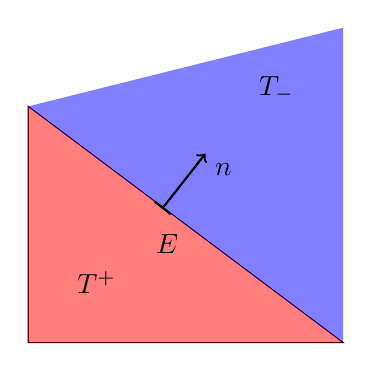
\begin{tikzpicture}[scale=1]
\coordinate (A) at (0,0);
\coordinate (C) at (0,3);
\coordinate (B) at (4,0);
\coordinate (D) at (4,4);
\coordinate (Tm) at (3.5,3.5);
\coordinate (Tp) at (0.5, 0.5);
\coordinate (e) at (1.5, 1.5);
\coordinate (start) at (1.7, 1.7);
\coordinate (end) at (2.25, 2.4);

\draw (A) -- (B) -- (C) -- cycle;
\fill[red, opacity=0.5] (A) -- (B) -- (C);
\fill[blue, opacity=0.5] (B) -- (C) -- (D);
\node[below left] at (Tm) {$T_{-} $ };
\node[above right] at (Tp) {$T^{+}$ };
\node[below right] at (e) {$E$ };

\draw [|->, thick] (start) -- (end);
% \node[above right] at (A) {A };
% \node[below right] at (B) {B};
% \node[above right] at (C) {C };
% \node[below right] at (D) {D};
\node[below right] at (end) {$n$};
\end{tikzpicture}
\caption{Edge $E \in \mathcal{F}_h $ shared by the triangles $T^{+}, T^{-} \in \mathcal{T}_{h} $ and the normal unit vector $n$.  }
    \label{fig:normal}
\end{figure}

 Thus, letting $u,v \in
H^{4}\left( T  \right) $ and using \eqref{eq:weak_form_identity_2}  does this hold ,

\begin{equation}
\label{eq:bi_basic_dg}
\left( \Delta  ^{2} u,v \right) _{T} =  \left( D^2u,D^2v \right) _{T } - \left<\partial _{nt} u, \partial _{t}v
\right>_{\partial T} - \left<\partial _{nn} u, \partial _{n}v \right>_{\partial T} + \left<\partial _{n} \nabla ^2 u,v
\right>_{\partial T}
.\end{equation}

For global continuity, let  $v \in V =  \left\{ v \in H^{1}\left( \Omega  \right): v_{T} \in  H^{4}\left( T \right), \ \forall T \in
\mathcal{T}_{h}    \right\}   \cap C^{0} (
\overline{\Omega }  ) $ and $u \in  H^{4}\left( \Omega  \right) $ such that,

\begin{equation}
\label{eq:bi_basic_dg2}
\left( \Delta  ^{2} u,v \right) _{\Omega } = \sum_{T \in  \mathcal{T} _{h}}^{} \left( D^2u,D^2v \right) _{T } - \left<\partial _{nt} u, \partial _{t}v
\right>_{\partial T} - \left<\partial _{nn} u, \partial _{n}v \right>_{\partial T} + \left<\partial _{n} \nabla ^2 u,v
\right>_{\partial T}
.\end{equation}

However, this can be simplified to

\begin{equation}
\label{eq:bi_basic_dg_full_1}
\begin{split}
\left( \Delta  ^{2} u, v \right) _{\Omega }
=& \sum_{T \in  \mathcal{T} _{h}}^{} \left( D^2u, D^2v \right)_{T}  + \sum_{E \in
\mathcal{F} ^{ext}_{}}^{} \left<\partial _{n} \nabla  ^2 u, v  \right> _{E}
- \left<\partial _{nt} u, \partial _{t} v \right> _{E}+
\left< \partial _{nn} u, \partial _{n} v \right>_{E} + \sum_{E \in \mathcal{F}  ^{int}}^{} \left<\partial _{nn} u , \jump{ \partial _{n} v }
\right>_{E} \\
& = \sum_{T \in  \mathcal{T} _{h}}^{} \left( D^2u, D^2v \right)_{T} + \sum_{E \in
\mathcal{F} ^{ext}_{}}^{} \left<g_{2 }, v  \right> _{E}
+ \left<n g_{2}, \nabla _{n}v \right>_{E} + \left<\partial _{t} g_{1} , \partial _{t}v \right>_{E}
+ \sum_{E \in \mathcal{F}  ^{int}}^{} \left< \partial _{nn} u    , \jump{ \partial_{n} v } \right>_{E}
\end{split}
\end{equation}
Where $\mathcal{F}^{int}_h , \mathcal{F} ^{ext}_{h} \subset \mathcal{F}_{h} $ be the set of interior and exterior facets of the triangulation $\mathcal{T}_{h} $.
Keep in mind that the jump over and edge $E$, visualized in figure \ref{fig:normal},   is defined as $\jump{ a } =    a^{+} - a^{-} $
and similarly will the mean be defined as $\mean{ a  } = \frac{1}{2}(   a^{+}
+ a^{-})$.  The equivalence of \eqref{eq:bi_basic_dg2} and \eqref{eq:bi_basic_dg_full_1} comes from the following argumentation.

\begin{equation*}
    \begin{split}
 \left( \Delta  ^{2} u,v \right) _{\Omega } & =\sum_{T\in \mathcal{T} _{h}}^{} \left( D^2u,D^2v \right) _{T } - \left<\partial _{nt} u, \partial _{t}v
\right>_{\partial T} - \left<\partial _{nn} u, \partial _{n}v \right>_{\partial T} + \left<\partial _{n} \nabla ^2 u,v
\right>_{\partial T} \\
&= \sum_{T\in \mathcal{T} _{h}}^{} \left( D^2u,D^2v \right) _{T } \\
&  \quad + \sum_{E \in \mathcal{F}_{h}^{ext} }^{} \underbrace{\left< \partial _{n} \nabla ^2 u, v  \right>_{E}}_{= \left< g_{2},v \right>_{E} }  -  \underbrace{\left<
\partial _{nt} u, \partial _{t} v \right> _{E}}_{= \left<\partial _{t} g_{1} , \partial _{t}v \right> }  - \underbrace{\left< \partial _{nn} u, \partial _{n} v \right>}_{= \left<n g_{2}, \partial  _{n}v \right>_{E}  }    \\
& \quad  + \sum_{E \in \mathcal{F} _{h}^{int}}^{} \underbrace{\left( \left<\partial _{n^{+}} \nabla ^2 u^{+}
        ,v^{+}\right>_{E}
+ \left<\partial _{n^{-}} \nabla ^2 u^{+} ,v^{-}\right>_{E}  \right)}_{(I)} +
\underbrace{\left( \left<\partial _{n^{+}t} u^{+}, \partial_{t} v^{+} \right>_{E} +  \left<\partial _{n^{-}t} u^{-},
        \partial_{t} v^{-}
\right>_{E}  \right) }_{(II)} +
\underbrace{\left( \left<\partial _{n^{+}n^{+}} u^{+}, v^{+} \right> _{E} + \left<\partial _{n^{-}n^{-}} u^{-}, v^{-}
\right> _{E} \right) }_{(III)}
    \end{split}
.\end{equation*}

Where integration over all interior edges $ \forall E \in \mathcal{F}_{h}^{int}$ is computed in this way:
\begin{equation*}
    \begin{split}
        (I) &  =    \left<\partial _{n^{+}} \nabla ^2 u^{+} ,v^{+}\right>_{E} +
        \left<\partial _{n^{-}} \nabla ^2 u^{+} ,v^{-}\right>_{E} =   \int_{E}^{}
        \jump{ \partial _{n} \nabla ^2 u \cdot v } =
         \int_{E}^{}
         \mean{ \partial _{n} \nabla ^2 u } \underbrace{\jump{ v }}_{= 0}    + \underbrace{\jump{ \partial _{n} \nabla ^2 u
         }}_{= 0}    \mean{ v } = 0 \\
        (II) &  =     \left<\partial _{n^{+}t} u^{+}, \partial_{t} v^{+}
        \right>_{E} +  \left<\partial _{n^{-}t} u^{-}, \partial_{t} v^{-}
\right>_{E}    =   \int_{E}^{}
        \jump{ \partial _{nt} u \cdot  \partial_{t} v } =
         \int_{E}^{}
         \mean{ \partial _{nt} u    } \underbrace{\jump{ \partial_{t} v }  }_{= 0}    + \underbrace{\jump{ \partial
                 _{nt}  u
         }}_{= 0}    \mean{ \partial _{t}v }  = 0\\
        (III) &  =     \left<\partial _{n^{+}n^{+}} u^{+}, \partial_{n^{+}} v^{+} \right>_{E} +  \left<\partial _{n^{-}n^{-}} u^{-}, \partial_{n^{-}} v^{-} \right>_{E}    =    \int_{E}^{} \jump{ \partial _{nn} u \cdot  \partial_{n} v } = \int_{E}^{}
        \mean{ \partial _{nn} u    } \underbrace{\jump{ \partial_{n} v }  }_{\neq 0}    + \underbrace{\jump{ \partial
                 _{nn}  u
         }}_{= 0}    \mean{ \partial _{n}v } =
        \left< \partial _{nn} u    , \jump{ \partial_{n} v } \right>_{E}  \\
    \end{split}
.\end{equation*}

Observe that the cancellations in the term $(I)$ appears of the continuity of $v\in V $ and $u\in H^{4}\left( \Omega  \right) $ which makes the jumps zero. For the second term $(II)$ does the terms become zero cancelled because the tangential derivative at the edge
has no jump. However, The third term $(III)$  is fairly interesting since the discontinuity in normal vector for $v \in V$ is a jump, while the second term is still continious. It can also be raised that $\mean{ \partial _{nn} u } = \partial _{nn} u  $ holds by the continuity of $H^{4}\left( \Omega  \right) $. Anyhow, the definition of jump of should more interesting when we later weakend the continuity of $u$ during discretization.
Hence, \eqref{eq:bi_basic_dg2} and \eqref{eq:bi_basic_dg_full_1} is equivalent.

We can finally start defining the fully discrete formulation. Let the basis be a $\mathcal{P}_{2} $ Lagrange finite element space so,
\[
V_{h} = \left\{ v \in C^{0}\left( \Omega  \right): v_{T} = v | _{T} \in P_{2}\left( T \right), \forall T \in
\mathcal{T}_{h}    \right\}
\]
and
\[
V_{h}^{*} = \begin{cases}
    V_{h} & \text{ if } \alpha  > 0 \\
    \left\{ v \in V_{h}: v\left( p_{*}  \right) = 0   \right\} &  \text{ if } \alpha   = 0
\end{cases}
\]
Now, if we choose $u \in V_{h}$ must we take account that the jump is discrete.
 We have now the final CP formulation.
The discretized numerical problem is to solve $w_{h} \in V_{h}^{*}$ such that
\begin{equation}
\label{eq:CP_A_F}
\mathcal{A}\left( w_{h}, v_{h} \right)   = F\left( v_{h} \right), \quad \forall v_{h} \in V_{h}^{*}  .
\end{equation}
where
\begin{equation}
\label{eq:CP_A_h_1}
\begin{split}
\mathcal{A} \left( w_{h}, v_{h} \right)   =&
  \quad  \left( \alpha  w_{h}, v_{h} \right) _{\Omega }\\
&  + \sum_{T \in \mathcal{T} _{h}}^{} \left( D^2 w_{h}, D^2v_{h} \right) _{T} \\
 & +
  \sum_{E \in \mathcal{F}_{h}^{int} }^{}
  \left< \mean{  \partial _{n n} w_{h} }, \jump{ \partial _{n }v_{h}} \right>_{E}  +
 \left< \mean{ \partial _{n n} v_{h} }, \jump{ \partial _{n}w }      \right>_{E}
+ \frac{\gamma}{h}  \left< \jump{ \partial _{n} w_{h}}, \jump{ \partial _{n} v_{h}   }   \right>_{E}
\end{split}
\end{equation}
and
\begin{equation}
\label{eq:CP_F_h}
F\left( v_{h} \right)  = \left( f, v_{h} \right) _{\Omega } +  \sum_ {\mathcal{F} ^{ext}_{}}^{} \left<g_{2 }, v_{h}  \right> _{E}
+ \left<n g_{2}, \partial  _{n}v_{h} \right>_{E} + \left<\partial _{t} g_{1} , \partial _{t}v_{h} \right>_{E}
\end{equation}
Notice that the regulation term termined by respectively a global tuning parameter $\gamma >0 $ and edge length $h = \left\lvert E \right\rvert $. Another key component to the formulation
in \eqref{eq:CP_A_h_1} after introduction of $ w_{h}, v_{h} \in V^{*}_{h}$  is that we expanded $\left< \partial _{nn}w, \jump{ \partial _{n} v }  \right>_{E} \to \left< \mean{ \partial _{nn}w_{h} }  , \jump{ \partial _{n} v_{h} }  \right>_{E} $ since we can longer not guarantee a
continious jump. For symmetric purposes we also added $ \left< \mean{ \partial _{nn} v_{h}}  , \jump{ \partial _{n} w_{h} }  \right>_{E} $.

We may introduce the compact notation of \eqref{eq:CP_A_h_1}.

\begin{equation}
\label{eq:CP_A_h}
\begin{split}
\mathcal{A} \left( w_{h}, v_{h} \right)   =&
  \quad  \left( \alpha  w_{h}, v_{h} \right) _{\Omega }\\
&  +  \left( D^2 w_{h}, D^2v_{h} \right) _{\mathcal{T} _{h}} \\
 & +
  \left< \mean{  \partial _{n n} w_{h} }, \jump{ \partial _{n }v_{h}} \right>_{\mathcal{F}_{h}}  +
 \left< \mean{ \partial _{n n} v_{h} }, \jump{ \partial _{n}w }      \right>_{\mathcal{F}_{h}}
+ \frac{\gamma }{h}  \left< \jump{ \partial _{n} w_{h}}, \jump{ \partial _{n} v_{h}   }   \right>_{\mathcal{F}_{h}}
\end{split}
\end{equation}

\subsection{Error and Stability Analysis of CP}%
\label{sub:error_and_stability_analysis_of_c0ip}

To guarantee convergence and stability we may want to check coercivity and boundedness of the method.

First of all, let us now establish some important inequalites.
\[
\begin{split}
    \textbf{Cauchy-Schwarz inequality: } & \| ab \|_{  }^{  }  \le \| a \|_{  }^{  } \| b \|_{  }^{  }   \\
    \textbf{Inverse inequality: } & \frac{1}{h}\| \partial _{nn}  v_{h} \|_{\mathcal{F}_{h}   }^{2  }  \le C_{j} \| \nabla ^2 v_{h} \|_{ \mathcal{T} _{h} }^{ 2 }   \\
    \textbf{Youngs epsilon inequality: } & 2ab =   2\sqrt{\varepsilon }a\cdot    \frac{b}{\sqrt{\varepsilon } } \le \varepsilon a^2+ b^2 \frac{1}{\varepsilon }
\end{split}
\]

Let the energy norm be on the form
\begin{equation}
\label{eq:A_energy_norm}
    \begin{split}
\| v_{h} \|_{ h }^{2  } & = \| v_{h} \|_{ a_{h} }^{ 2 } =  \|  w_{h} \|_{ \Omega  }^{  }\| v_{h} \|_{ \Omega  }^{  }  +  \| \nabla ^2 v_{h} \|_{ \mathcal{T} _{h}  }^{ 2 }  + \|  h^{-\frac{1}{2}} \jump{ \partial _{n} v_{h}    }\|_{  \mathcal{F} _{h} }^{  } \\
\| v \|_{ h }^{ 2 }  &= \| v \|_{ a_{h},* }^{ 2 } = \| v \|_{ a_{h} }^{ 2 }  + \| h^{\frac{1}{2}} \left\{ \partial _{nn } v\right\}  \|_{ F  }^{  }, \quad  v\in V \oplus V_{h}
    \end{split}
.\end{equation}
The method is said to be coercive if $\mathcal{A} _{h}\left( v_{h}, v_{h} \right) \ge  C \| v_{h} \|_{ a_{h} }^{  } $. Similarly, it is bounded if $ \mathcal{A} _{h} \left( v_{h}, u_{h} \right) \le  C \| u_{h} \|_{  a_{h}}^{ 2 }  \| v_{h} \|_{ a_{h}
}^{ 2 } $ and then, according to Lax Milgram (need reference), the solution does exist and be unique.

\subsubsection{Coercitivity}%
\label{ssub:coercitivity}


Suppose we have the CP problem described in \eqref{eq:CP_A_F}. Then is the coercivity be computed such that
\[
    \begin{split}
\mathcal{A} \left( v_{h}, v_{h} \right) & =\alpha \|  w_{h}  v_{h} \|_{ \Omega  }^{  } +  \| D^2v_{h} \|_{ \mathcal{T} _{h} }^{2  }  + 2 \left(  \mean{ \partial _{nn} v_{h} }    ,  \jump{ \partial _{n}v_{h} }     \right) _{\mathcal{F} _{h}} +  \frac{\gamma}{h} \|  \jump{ \partial _{n} v_{h} }
  \|_{ \mathcal{F} _{h} }^{ 2 } \\
\quad \textit{Cauchy-Schwarz inequality} \quad
& \ge \alpha \| w_{h}  \|_{\Omega   }^{  } \| v_{h} \|_{\Omega   }^{  } +   \| \nabla ^2 v_{h} \|_{ \mathcal{T} _{h} }^{2  } -2 \| h^{\frac{1}{2}} \mean{ \partial _{nn}v_{h} }    \|_{  \mathcal{F} _{h}}^{  } \| h^{-\frac{1}{2}} \jump{ \partial _{n}v_{h} }    \|_{  \mathcal{F} _{h}}^{  } + \gamma \| h^{-\frac{1}{2}}  \jump{ \partial _{n}v_{h} }   \|_{ \mathcal{F} _{h}  }^{ 2 } \\
\quad \textit{Inverse inequality} \quad
 &  \ge \alpha \| w_{h}  \|_{\Omega   }^{  } \| v_{h} \|_{\Omega   }^{  } + \| \nabla ^2 v_{h}  \|_{ \mathcal{T} _{h}  }^{ 2  } - 2 C^{\frac{1}{2}}_{j} \|   \nabla ^2 v_{h}    \|_{ \mathcal{T} _{h}  }^{  } \| h^{-\frac{1}{2}} \jump{ \partial _{n} v_{h} }   \|_{ \mathcal{F} _{h} }^{  }  + \gamma \| h^{ -\frac{1}{2}} \jump{
 \partial _{n } v_{h}}   \|_{ \mathcal{F}_{h}}^{2}  \\
\quad \textit{ Youngs epsilon inequality} \quad
  &  \ge\alpha \| w_{h}  \|_{\Omega   }^{  } \| v_{h} \|_{\Omega   }^{  } +  \| \nabla ^2 v_{h} \|_{ \mathcal{T}_{h}  }^{2  } - \varepsilon C_{j} \| \nabla ^2 v_{h} \|_{ \mathcal{T} _{h} }^{2  } - \frac{1}{\varepsilon } \| h^{\frac{1}{2}} \jump{ \partial _{n} v_{h} }   \|_{ \mathcal{F} _{h} }^{2  }  + \gamma \|
  h^{-\frac{1}{2}} \jump{ \partial _{n} v_{h}}   \|_{ \mathcal{F} _{h} }^{2  }  \\
  & =  \alpha \| w_{h}  \|_{\Omega   }^{  } \| v_{h} \|_{\Omega   }^{  } +\left( 1 - \varepsilon C_{j} \right) \| \nabla ^2 v_{h} \|_{  }^{ 2 } + \left( \gamma  - \frac{1}{\varepsilon } \right) \| h^{-\frac{1}{2}} \jump{ \partial _{n} v_{h} }   \|_{ \mathcal{T} _{h} }^{ 2 } \\
  (\varepsilon  = \frac{1}{2 C_{j} })  \implies  \quad \quad &= \alpha \| w_{h}  \|_{\Omega   }^{  } \| v_{h} \|_{\Omega   }^{  } +\frac{1}{2} \| \nabla ^2 v_{h} \|_{ \mathcal{T} _{h} }^{ 2 }  + \underbrace{\left( \gamma -2 C_{j} \right)}_{ \ge  \frac{1}{2}}  \| h^{\frac{1}{2}} \jump{ \partial _{n} v_{h} }   \|_{
  \mathcal{F} _{h} }^{  } \ge C \| v_{h} \|_{ a_{h} }^{  2}
    \end{split}
\]
This holds if $C=\min\left\{  \alpha , 1 /2\right\}$.
Observe that for the first inequality is the standard \textbf{Cauchy-Schwarz inequality} such that $$\left( \mean{ \partial_{nn} v_{h} }  , \jump{ \partial _{n} v_{h} }   \right) _{\mathcal{F} _{h}} \ge - \| h^{-\frac{1}{2}} \mean{ \partial _{nn}
v_{h} }    \|_{\mathcal{F}_{h}   }^{  } \| \mean{ \partial _{n}v_{h} }   \|_{ \mathcal{F}_{h}   }^{  } .  $$ On the second inequality the \textbf{Inverse inequality} was applied,
\[
- \| h^{\frac{1}{2}} \mean{ \partial _{nn}v }   \|_{ \mathcal{F} _{h}  }^{  }\ge - C_{j}^{\frac{1}{2}} \| \nabla ^2 v_{h} \|_{ \mathcal{T} _{h} }^{  }
\]
The next step is then to use the \textbf{Youngs epsilon inequality} to be able to seperate the facets and triangulation norms. \[
 - 2 C^{\frac{1}{2}}_{j} \|  \nabla ^2 v_{h}    \|_{ \mathcal{T} _{h}  }^{  } \| h^{\frac{1}{2}} \jump{ \partial _{n} v_{h} }   \|_{ \mathcal{F} _{h} }^{2  } \ge- \varepsilon C_{j} \| \nabla ^2 v_{h} \|_{ \mathcal{T} _{h} }^{2  } -
 \frac{1}{\varepsilon } \| h^{\frac{1}{2}} \jump{ \partial _{n} v_{h} }   \|_{ \mathcal{F} _{h} }^{2  }
\]
The last step was to choose a $\varepsilon $ and $\gamma $ as some positive constant so that the second term is restricted to be multiplied with something bigger than $\frac{1}{2}$. Thus, the term fulfils coercivity of the \eqref{eq:A_energy_norm}. Hence, the CP method is coercive.

\subsubsection{Boundedness}%
\label{ssub:bounded}
We want the CP method to be bounded.
\begin{equation*}
    \begin{split}
\mathcal{A} \left( w_{h}, v_{h} \right)   =& \left( \alpha w_{h}, v_{h} \right) _{\Omega } +
    \left( \nabla ^2 w_{h}, \nabla ^2v_{h} \right) _{\mathcal{T} _{h}}
  +
  \left< \mean{  \partial _{n n} w_{h} }, \jump{ \partial _{n }v_{h}} \right>_{\mathcal{F}_{h}}  +
 \left< \mean{ \partial _{n n} v_{h} }, \jump{ \partial _{n}w }      \right>_{\mathcal{F}_{h}}
+ \frac{\gamma }{h}  \left< \jump{ \partial _{n} w_{h}}, \jump{ \partial _{n} v_{h}   }   \right>_{\mathcal{F}_{h}} \\
\quad \textit{Cauchy-Schwarz inequality }\quad  &\le \alpha  \|  w_{h} \|_{\Omega   }^{  } \| v_{h} \|_{ \Omega  }^{  }     +
\| \nabla ^2w_{h} \|_{\mathcal{T} _{h}   }^{  }  \| \nabla ^2v_{h} \|_{\mathcal{T} _{h}   }^{  } + \| h^{\frac{1}{2}}\mean{ \partial _{nn} w_{h} } \|_{ \mathcal{F}_{h}  }^{  } \| h^{-\frac{1}{2}}\jump{ \partial _{n} v_{h} } \|_{ \mathcal{F}_{h}  }^{  }    \\
& \quad  + \| h^{\frac{1}{2}}\mean{ \partial _{nn} v_{h} }
\|_{ \mathcal{F}_{h}  }^{  } \| h^{-\frac{1}{2}}\jump{ \partial _{n} w_{h} } \|_{ \mathcal{F}_{h}  }^{  } + \gamma \| h^{-1} \jump{ \partial _{n} v_{h}}   \|_{ \mathcal{F} _{h} }^{  }   \|  \jump{ \partial _{n} w_{h}}   \|_{ \mathcal{F} _{h} }^{  } \\
\quad \textit{Inverse inequality }\quad  &\le \alpha  \|  w_{h} \|_{\Omega   }^{  } \| v_{h} \|_{ \Omega  }^{  }  +
\| \nabla ^2w_{h} \|_{\mathcal{T} _{h}   }^{  }  \| \nabla ^2v_{h} \|_{\mathcal{T} _{h}   }^{  } + C_{j}^{\frac{1}{2}} \| \nabla ^2 w_{h} \|_{\mathcal{T} _{h}  }^{  }  \| h^{-\frac{1}{2}}\jump{ \partial _{n} v_{h} } \|_{ \mathcal{F}_{h}  }^{  }   +
 \\
& \quad  C_{j}^{\frac{1}{2}} \| \nabla ^2 w_{h} \|_{\mathcal{T} _{h}  }^{  }
 \| h^{-\frac{1}{2}}\jump{ \partial _{n} w_{h} } \|_{ \mathcal{F}_{h}  }^{  } + \gamma \| h^{-1} \jump{ \partial _{n} v_{h}}   \|_{ \mathcal{F} _{h} }^{  }   \|  \jump{ \partial _{n} w_{h}}   \|_{ \mathcal{F} _{h} }^{  } \\
\textit{ Using \eqref{eq:bounded_ineq}}  \quad & \le\alpha  \|  w_{h} \|_{a_{h}   }^{  } \| v_{h} \|_{ a_{h}   }^{  } + \| w_{h} \|_{ a_{h} }^{  } \| v_{h} \|_{ a_{h} }^{  }  + 2C_{j}^{\frac{1}{2}} \| w_{h} \|_{ a_{h} }^{  } \| v_{h} \|_{ a_{h} }^{  } + \gamma \| v_{h} \|_{ a_{h} }^{  } \| w_{h} \|_{ a_{h} }^{  } \\
& \le  \left( \alpha + 1 + 2C_{j}^{\frac{1}{2}} + \gamma  \right)  \| v_{h} \|_{a_{h}  }^{  }  \| w_{h} \|_{ a_{h} }^{  }  \le  K  \| v_{h} \|_{a_{h}  }^{  }  \| w_{h} \|_{ a_{h} }^{  }
\end{split}
\end{equation*}

Thus, the CP method is shown to be bounded.
Again, the first step was to apply the \textbf{Cauchy-Schwarz inequality} for every term. On the second inequality the \textbf{Inverse inequality} was applied so that
\[
\| h^{\frac{1}{2}} \mean{ \partial _{nn}v_{h} }   \|_{ \mathcal{F} _{h}  }^{  }\le   C_{j}^{\frac{1}{2}} \| \nabla ^2 v_{h} \|_{ \mathcal{T} _{h} }^{  } \quad \text{and} \quad   \| h^{\frac{1}{2}} \mean{ \partial _{nn}w_{h} }   \|_{ \mathcal{F} _{h}
}^{  }\le   C_{j}^{\frac{1}{2}} \| \nabla ^2 w_{h} \|_{ \mathcal{T} _{h} }^{  }.
\]
The second step can we luckily observe that all terms invidually is less than the norm such that
\begin{equation}
\label{eq:bounded_ineq}
\begin{split}
\| w_{h} \|_{\Omega    }^{  }  \| v_{h} \|_{ \Omega    }^{  } & \le \| w_{h} \|_{ a_{h} }^{  } \| v_{h} \|_{ a_{h} }^{  }, \\
\| \nabla ^2w_{h} \|_{\mathcal{T}_{h}   }^{  }  \| \nabla ^2v_{h} \|_{\mathcal{T}_{h}   }^{  } & \le \| w_{h} \|_{ a_{h} }^{  } \| v_{h} \|_{ a_{h} }^{  }, \\
\|  \nabla ^2 w_{h} \|_{ \mathcal{T} _{h} }^{ } \| h^{-\frac{1}{2}} \jump{ \partial _{n} v_{h} }   \|_{ \mathcal{F} _{h} }^{  }  & \le  \| w_{h} \|_{ a_{h} }^{  } \| v_{h} \|_{ a_{h} }^{  }, \quad  \|  \nabla
^2 v_{h} \|_{ \mathcal{T} _{h} }^{ } \| h^{-\frac{1}{2}} \jump{ \partial _{n} w_{h} }   \|_{ \mathcal{F} _{h} }^{  }   \le \| v_{h} \|_{ a_{h} }^{  } \| w_{h} \|_{ a_{h} }^{  }, \\
\text{and} \quad    \gamma \| h^{-1 } \jump{ \partial _{n} v_{h} }   & \|_{ \mathcal{F} _{h}  }^{  }  \| \jump{ \partial _{n} w_{h} }    \|_{\mathcal{F}_{h}   }^{  }   \le \gamma \| v_{h} \|_{ a_{h} }^{  }  \| w_{h} \|_{ a_{h} }^{  }.
\end{split}
\end{equation}

Hence, the CP method is does fulfills the Lax Milgram criteria because it is both bounded and unique.


\section{HCP Method copied from NGSolve}%
\label{ssub:hc0ip_method_from_ngsolve}

We consider the Kirchhoff plate equation: Find $w \in H^2$, such that

$$
\int \nabla^2 w : \nabla^2 v = \int f v
$$

A conforming method requires $C^1$ continuous finite elements. But there is no good option available, and thus there is no $H^2$ conforming finite element space in NGSolve.

$$
\sum_T \nabla^2 w : \nabla^2 v
- \int_{E} \{\nabla^2 w\}_{nn} \, [\partial_n v]
- \int_{E} \{\nabla^2 v\}_{nn} \, [\partial_n w] + \alpha \int_E  [\partial_n w]  [\partial_n v]
$$

[Baker 77, Brenner Gudi Sung, 2010]

We consider its hybrid DG version, where the normal derivative is a new, facet-based variable:


$$
\sum_T \nabla^2 w : \nabla^2 v
- \int_{\partial T} (\nabla^2 w)_{nn} \, (\partial_n v - \widehat{v_n})
- \int_{\partial T} (\nabla^2 v)_{nn} \, (\partial_n w - \widehat{w_n}) + \alpha \int_E (\partial_n v - \widehat{v_n}) (\partial_n w - \widehat{w_n})
$$






